\section{Graphs in LabVIEW Simulation Module}  

\begin{figure}[h!]
\centering
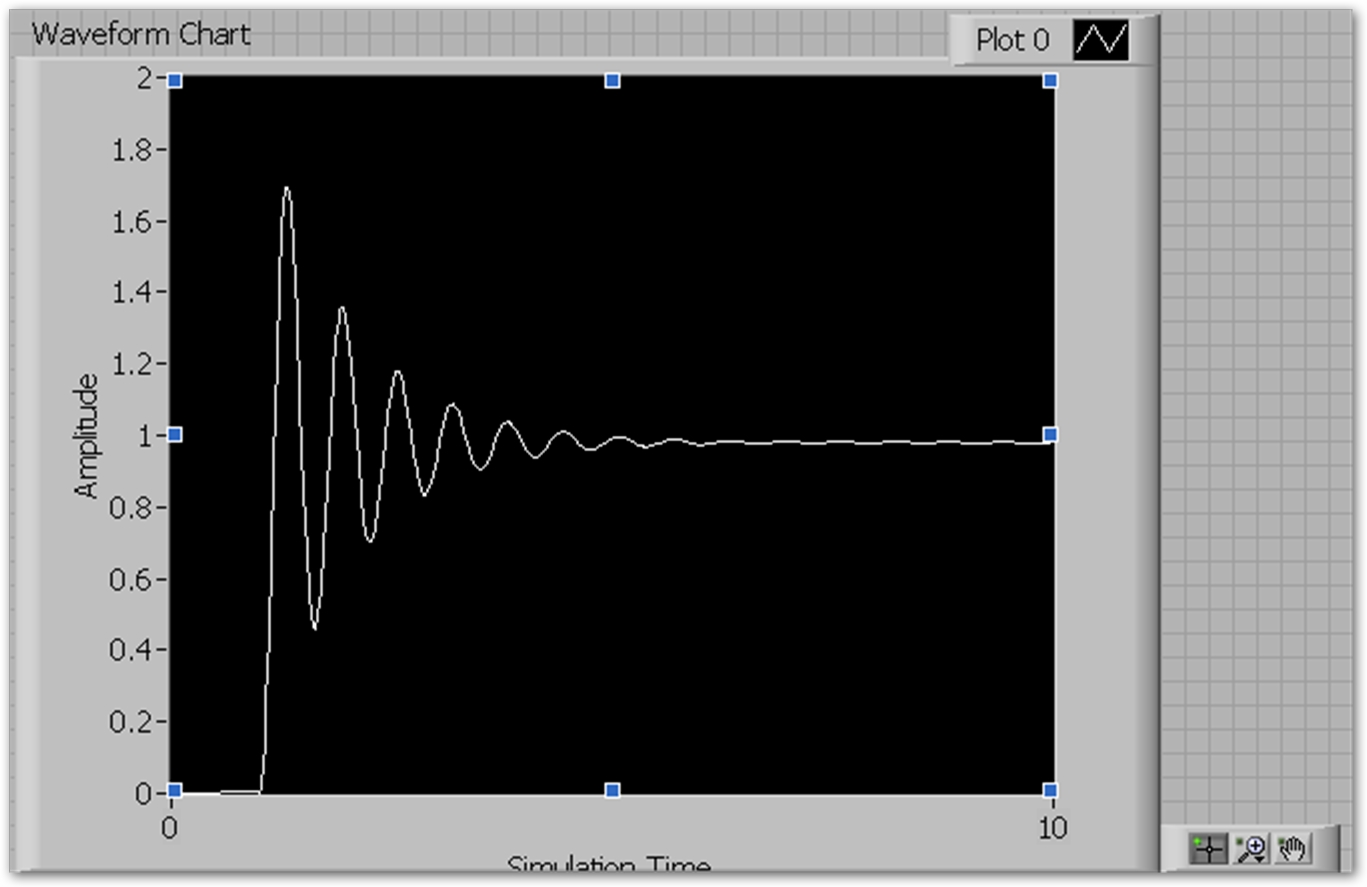
\includegraphics[width=6in]{graphs/waveform1}
\caption{A Sim-Time Waveform}
\label{fig-simtimewaveform}
\end{figure}

Graphs are typically created using a sim-time waveform (in the simulation
module), as seen in Fig.\ref{fig-simtimewaveform}.  However, if you want trace
functionality, the you should use the XY Graph (also in the simulation module).
The back panel for this is seen in Fig.~\ref{fig-xygraphback}.  Note that the XY
Graph requires both time (which we generate in this case using a ramp function)
and the actual signal, which are then plotted against each other.  In order to
plot them both, one must ``bundle'' the two signals together using a bundle
block (located in the ``Cluster and Variant'' palette).  

The cursor is created in the front panel (see Fig.~\ref{fig-xygraphfront}) by
right clicking on the graph and selecting \emph{Properties}.  Then select
cursor, choose to add a cursor, and a cursor will show up on the graph.  Note
that the cursor can only select actual data points\textendash it will not interpolate.
Therefore, you may wish to select a maximum step size in your integration
algorithm that makes it move smoothly from point to point.  (E.g., reduce the
maximum step size.)

\begin{figure}[h!]
\centering
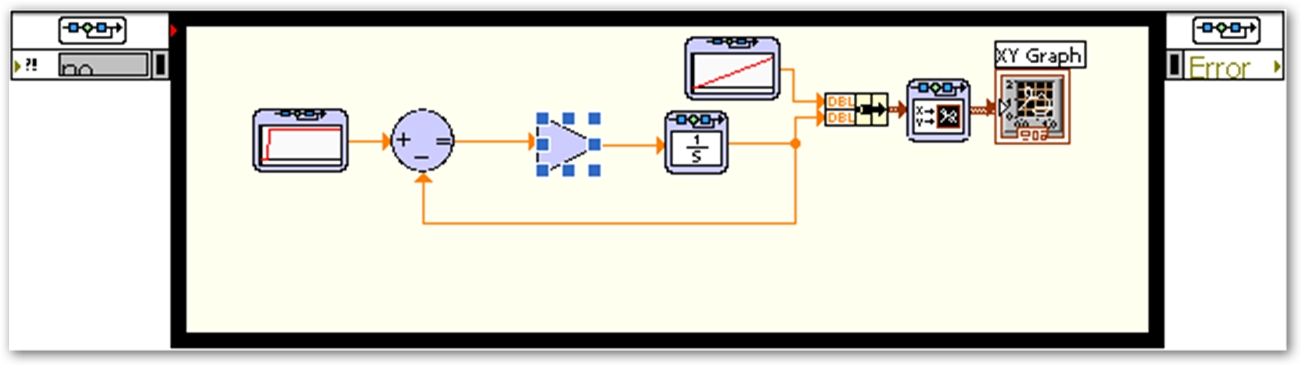
\includegraphics[width=6in]{graphs/xygraphback}
\caption{An XY Graph Back Panel}
\label{fig-xygraphback}
\end{figure}

\begin{figure}[h!]
\centering
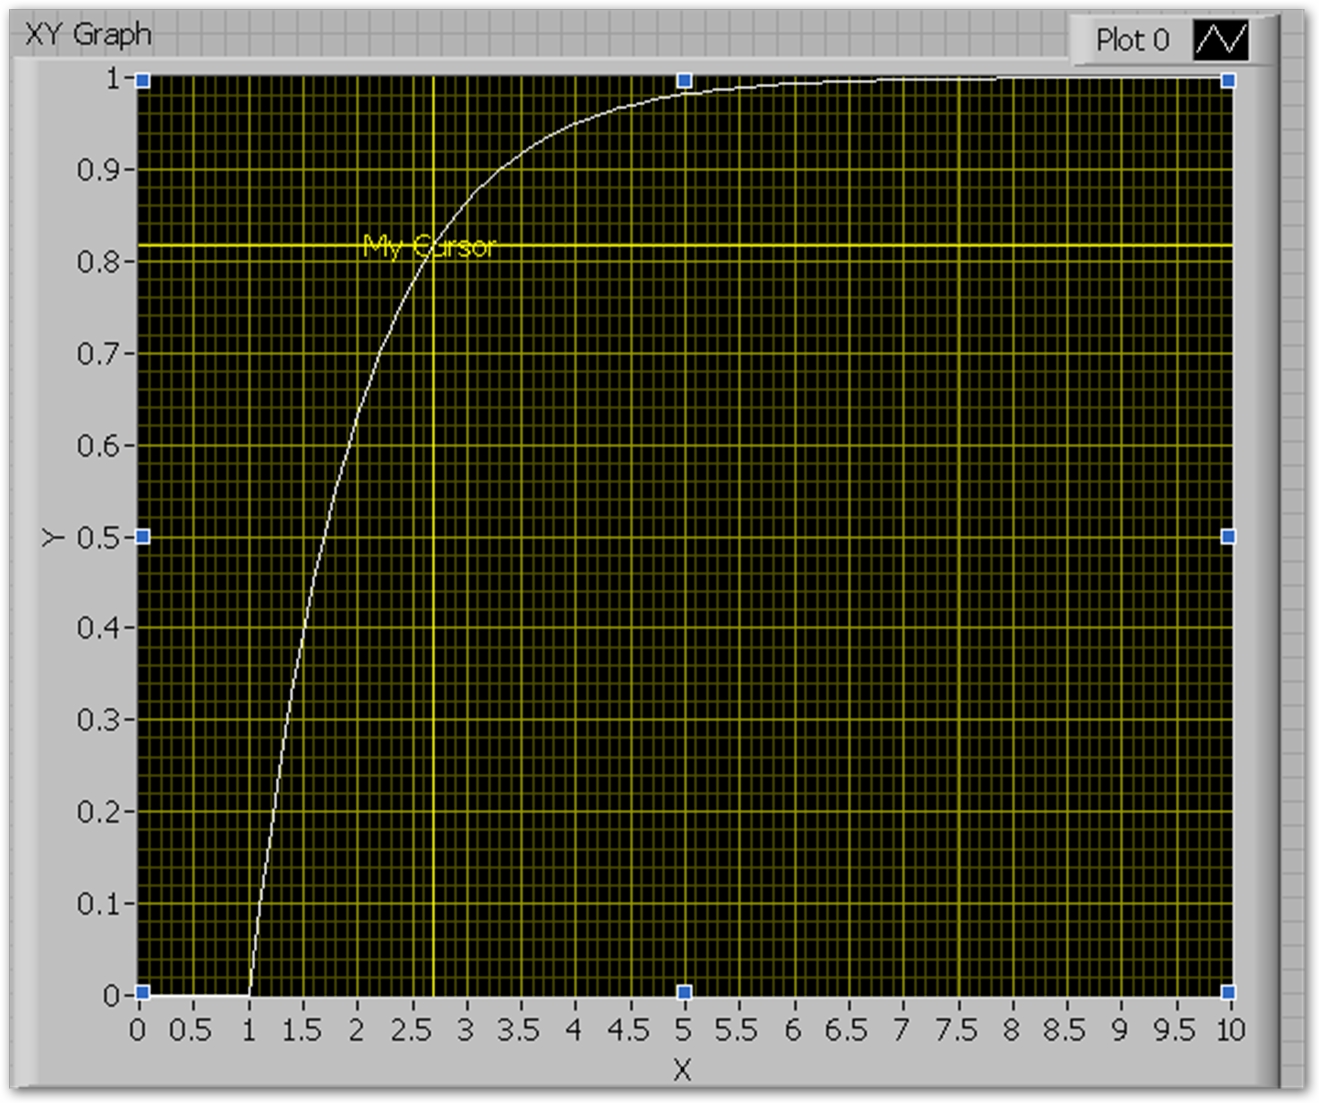
\includegraphics[width=6in]{graphs/xygraphfront}
\caption{A XY Graph Front Panel with Cursor}
\label{fig-xygraphfront}
\end{figure}

\subsection{Some Notes on Graphing in LabVIEW}

\begin{enumerate}
\item There are two distinct types of XY Graphs.  One is the Simulation Module
  ``Buffer XY graph'' (found in the Simulation Module Palette under ``Graph
  Utilities'') that \emph{can only be used in the simulation module}.  The other
  is the standard XY graph that can be found under the ``Graph'' pallette of the
  \emph{front panel}.  (I.e., you find it by right-clicking on the front panel,
  select the ``Graph'' palette, and then click on ``XY Graph.'')
\item The default amount of data a Waveform Chart in the Simulation Module
  displays is 1024.  If your time steps are too small in a simulation or
  experiment, you may not get all your data.  Hence, if this happens you should
  change the ``Chart History Length'' to a larger number (by right clicking on
  the graph).
\item Lastly, the time axis sometimes gets set to Day/Year format.  If this
  happens, go into ``Properties'' and under ``Format and Precision'' set Type to
  SI notation.
\end{enumerate}

%% Local Variables:
%% TeX-master: "../LVmanual.tex"
%% End:

